% !TEX TS-program = pdflatex --shell-escape
%\documentclass[handout]{beamer} %slides+notes only
%\documentclass[10pt,t]{beamer} %slides only
% The laulatex is being updated. The following RequirePackage line is needed for now.
%
% Under Menu, select compiler 2017 (Legacy) to get animate to make a pdf with a working animation.
% The 2019 compiler does not work as of 18 September 2020.
%
% Hold down the wheel or middle mouse button pause the animation.
% Add the control keyword to see the controls.
%
\documentclass[aspectratio=169]{beamer}
\RequirePackage{luatex85}
\usepackage{animate}
\usepackage{pgfpages}
\usepackage{moresize}
\usetheme{default}
\beamertemplatenavigationsymbolsempty
\hypersetup{pdfpagemode=UseNone} % don't show bookmarks on initial view
%tables
\usepackage{booktabs}% http://ctan.org/pkg/booktabs
% font
\usepackage{amsmath}
\usepackage{amssymb}
\usepackage{minted}
\usepackage{fix-cm}
\usepackage{fontspec}
\usepackage{gensymb}
\usepackage{tabularx,booktabs}


\usepackage{enumitem}

\newminted{python}{fontsize=\normalsize, 
                   linenos=false,
                   numbersep=8pt,
                   gobble=4,
                   breaklines,
                   frame=lines,
                   bgcolor=bgpython,
                   framesep=3mm}

\newminted{bash}{fontsize=\largesize, 
                   linenos=false,
                   numbersep=8pt,
                   breaklines,
                   gobble=4,
                   frame=lines,
                   bgcolor=bgbash,
                   framesep=3mm}

\definecolor{bgpython}{rgb}{0.95,0.95,0.95}
\definecolor{bgbash}{rgb}{0.95,0.85,0.75}

\setsansfont{TeX Gyre Heros}
\setbeamerfont{note page}{family*=pplx,size=\footnotesize} % Palatino for notes
% "TeX Gyre Heros can be used as a replacement for Helvetica"
% In Unix, unzip the following into ~/.fonts
% In Mac, unzip it, double-click the .otf files, and install using "FontBook"
%   http://www.gust.org.pl/projects/e-foundry/tex-gyre/heros/qhv2.004otf.zip

% Center the title and increase its size
\setbeamertemplate{frametitle}[default][center]
\setbeamerfont{frametitle}{size=\huge}


% named colors
\definecolor{offwhite}{RGB}{249,242,255}
\definecolor{foreground}{RGB}{25,25,25}
\definecolor{background}{RGB}{255,255,255}
\definecolor{title}{RGB}{100,0,0}
\definecolor{gray}{RGB}{155,155,155}
\definecolor{subtitle}{RGB}{50,0,0}
\definecolor{hilight}{RGB}{102,255,204}
\definecolor{vhilight}{RGB}{255,111,207}
\definecolor{lolight}{RGB}{155,155,155}
%\definecolor{green}{RGB}{125,250,125}

% use those colors
\setbeamercolor{titlelike}{fg=title}
\setbeamercolor{subtitle}{fg=subtitle}
\setbeamercolor{institute}{fg=gray}
\setbeamercolor{normal text}{fg=foreground,bg=background}
\setbeamercolor{item}{fg=foreground} % color of bullets
\setbeamercolor{subitem}{fg=gray}
\setbeamercolor{itemize/enumerate subbody}{fg=gray}
\setbeamertemplate{itemize subitem}{{\textendash}}
\setbeamerfont{itemize/enumerate subbody}{size=\footnotesize}
\setbeamerfont{itemize/enumerate subitem}{size=\footnotesize}

% page number
\setbeamertemplate{footline}{%
    \raisebox{5pt}{\makebox[\paperwidth]{\hfill\makebox[20pt]{\color{gray}
          \scriptsize\insertframenumber}}}\hspace*{5pt}}

% add a bit of space at the top of the notes page
\addtobeamertemplate{note page}{\setlength{\parskip}{12pt}}

% a few macros
\newcommand{\bi}{\begin{itemize}}
\newcommand{\ei}{\end{itemize}}
\newcommand{\ig}{\includegraphics}
\newcommand{\subt}[1]{{\footnotesize \color{subtitle} {#1}}}

\usepackage{latexsym} % for squares for the check-list environment
\newenvironment{checklist}{%
  \begin{list}{}{}% whatever you want the list to be
  \let\olditem\item
  \renewcommand\item{\olditem[$\Box$] }
}{%
  \end{list}
}


% title info
\title{Title of Group Meeting, Journal Club, Workshop, Platform Talk, Seminar, or Lecture} 
\author{\textbf{Blaine Mooers, PhD \\ blaine-mooers@ouhsc.edu \\ 405-271-8300}}
\institute{{Department of Biochemistry \& Molecular Biology}\\[2pt]{University of Oklahoma Health Sciences Center, Oklahoma City} }
% to hide auto date,use \date{}
\date{Super-duper Cool Workshop in Parallel Universe\\ 16 September 2022}


\begin{document}

% title slide
\section{Title slide}
{
\setbeamertemplate{footline}{} % no page number here
\frame{
  \titlepage
  \note{

} } }
\note{
7:06
Hi, I am Blaine Mooers.
I will be talking about 
I am an associate professor of Biochemistry and Molecular Biology at the University of Oklahoma Health Sciences Center in Oklahoma City.
}



%%%%%%%%%%%%%%%%%%%%%%%%%%%%%%%%%%%%%%%%%%%%   2   %%%%%%%%%%%%%%%%%%%%%%%%%%%%%%%%%%%%%%%%%%%%    
% Slide 2
\section{Sample imported PNG file}
\begin{frame}
\frametitle{Sample imported PNG file}
\begin{center}
    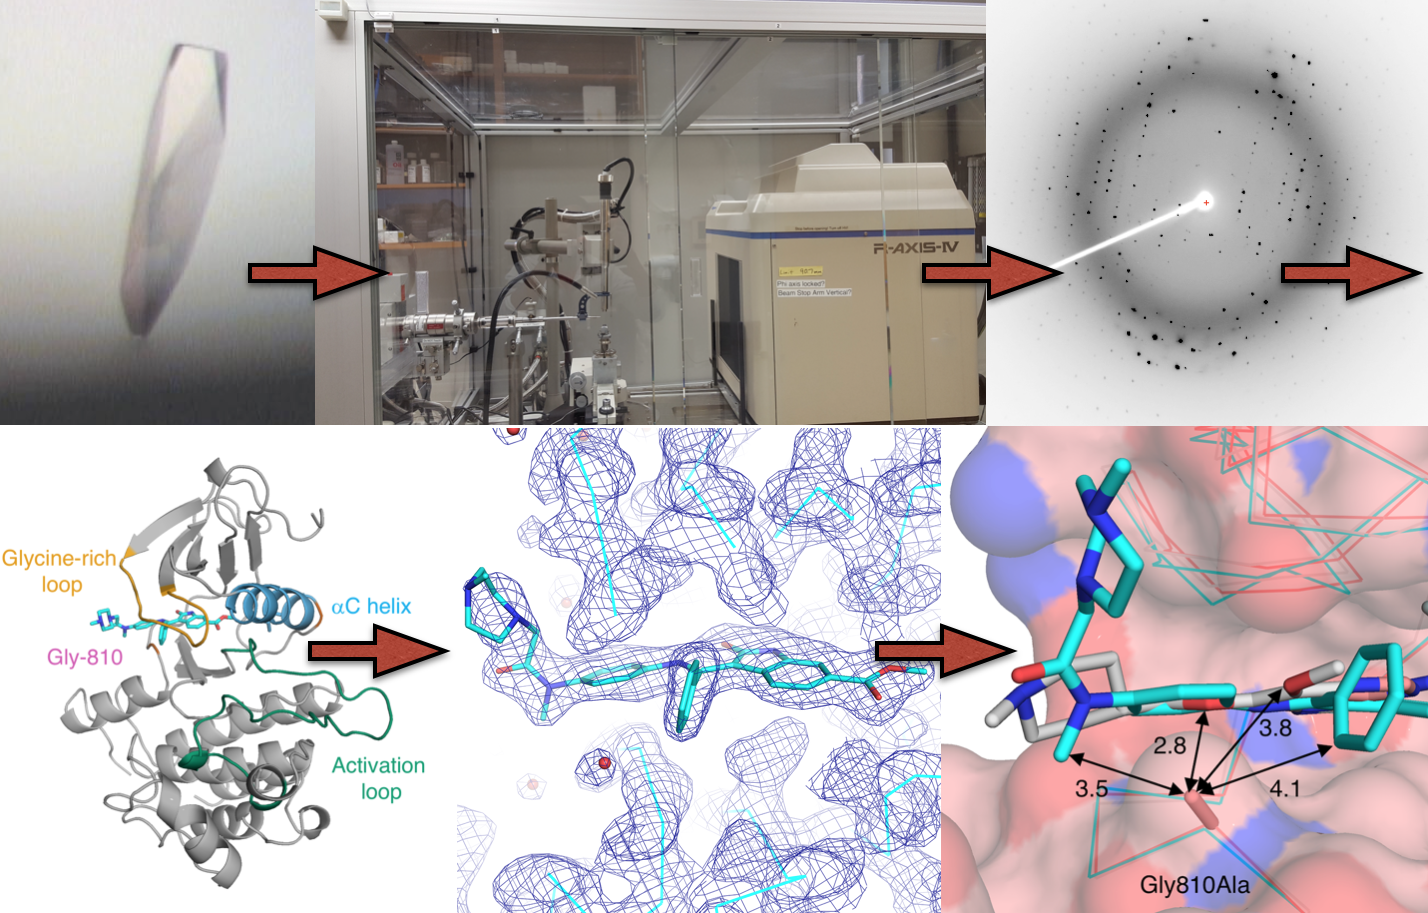
\includegraphics[width=0.79\textwidth, angle=0]{./Figures/workflow}
\end{center}
\end{frame}
\note{
PNG and PDF files work best. SVG and EPS are possible. Tiff do not import.
}




%%%%%%%%%%%%%%%%%%% 6 df  %%%%%%%%%%%%%%%%%%%%%%%%%%    
% Slide 6
\section{Itemized list with custom bullets}
\begin{frame}
\frametitle{Itemized list with custom bullets}
\Large{
% requires the enumitem package
\begin{itemize}[font=$\bullet$\scshape\bfseries]
    \item Org supports literate programming via code blocks.
    \item Org can run PyMOL through PyMOL's Python API.
    \item Org file can serve as a gallery of draft images.
    \item Submit Org file as supplemental material.
    \item Can include in electronic diary.
\end{itemize}
}
\end{frame}
\note{

}


% Slide 2
\section{Multi-line equation}
\begin{frame}
\frametitle{Multi-line equation}
\Large{
\begin{center}
\begin{equation}
\begin{aligned}
y_{i} & \sim \operatorname{Normal}\left(\mu_{i}, \sigma\right) \\
\mu_{i} &=\alpha+\beta x_{i} \\
\alpha & \sim \operatorname{Normal}(0,100) \\
\beta & \sim \operatorname{Normal}(0,1) \\
\sigma & \sim \operatorname{Exponential}(1)
\end{aligned}
\end{equation}
\end{center}
}
\end{frame}
\note{}





%%%%%%%%%%%%%%%%%%%%%%%% 11 %%%%%%%%%%%%%%%%%%%%%%%%%%%%%%%%%%%    
% Slide 11
\section{Sample table}
\begin{frame}
\frametitle{Sample table}

\begin{center}
    %\includegraphics[width=0.86\textwidth, angle=0]{./Figures/plusMinus.png}
\begin{center}
\begin{large}
\begin{tabular}{lcc}
\toprule
\textbf{Features} & \textbf{Org Mode} & \textbf{Jupyter}\\
\midrule
Tab triggers & +++ & - \\
Tab stops & +++ & -\\
Snippet groups & +++ & +\\
Parallel sessions in same document & + & -\\
Rendering speed & -- & ++ \\
Scrolling speed & -- & ++\\
Ease and speed to PDF & +++++ & + \\
\bottomrule
\end{tabular}
\end{large}
\end{center}    
    
    
\end{center}

\end{frame}
\note{
The notes field can be printed with the slide on the same page.
Uncomment line 2 and comment line 12.
}


\section{Code block with syntax highlighting (1/2)}
\defverbatim[colored]\exampleCodeC{
\large{
\begin{pythoncode}
    #+BEGIN_SRC emacs-lisp :results value scalar
    (* 40 1000 1000 1000 1000 1000 1000 1000)
    #+END_SRC
    #+RESULTS:
    : 40000000000000000000
\end{pythoncode}
}
}
% Slide 24
\begin{frame}
\frametitle{Code block with syntax highlighting (1/2)}
\Large{
Place cursor inside code block and enter C-c C-c to run the code. 
In this case, it is defined for the pythoncode environment. You can also use footnotes in slides \footnote{Note that the color of the background is defined in the Preamble.}.}
\exampleCodeC
\end{frame}


\section{Code block with different background color (2/2)}
\defverbatim[colored]\exampleCodeC{
\large{
\begin{bashcode}
    #+BEGIN_SRC emacs-lisp :results value scalar
    (* 40 1000 1000 1000 1000 1000 1000 1000)
    #+END_SRC
    #+RESULTS:
    : 40000000000000000000
\end{bashcode}
}
}
% Slide 24
\begin{frame}
\frametitle{Code block with different background color (2/2)}
\exampleCodeC
\large{
Note that the color of the background is defined in the Preamble.
In this case, it is defined for the bashcode environment.
}
\end{frame}

%%%%%%%%%%%%%%%%%%%%%%%%%%%%%%%%%%%%%%%%%%%%   28   %%%%%%%%%%%%%%%%%%%%%%%%%%%%%%%%%%%%%%%%%%%%    
% Slide 12
\section{Acknowledgements}
\begin{frame}
\frametitle{Acknowledgements}
\Large{
\begin{itemize}[font=$\bullet$\scshape\bfseries]
    \item Nathan Shock Data Science Workshop
\end{itemize}
\vspace{2mm}
Funding:
\begin{itemize}[font=$\bullet$\scshape\bfseries]
    \item Warren Delano Memorial Open-Source PyMOL Fellowship
    \item NIH: R01 CA242845, R01 AI088011
    \item NIH: P20 GM103640, P30 CA225520, P30 AG050911-07S1 
    \item OCAST HR20-002
    \item PHF Team Science Grant
\end{itemize}
}
\end{frame}
\note{
I would like to thank feedback on this project from our local Data Science Workshop that meets once a month.
I would also like to thank these funding sources that supported this work.
}

\end{document}

    



